\documentclass[10pt]{article}
\usepackage[dvipsnames]{xcolor}
\usepackage{tikz}
\usepackage[obeyspaces]{url}
\usepackage{multicol}
\usepackage{xspace}
\usepackage{pstricks}
\usepackage{wrapfig}
\usepackage[section]{placeins}
\usepackage{wrapfig}
\usepackage[default]{droidserif}
\usepackage[T1]{fontenc}

\usepackage{listings}

\newcommand{\todo}[1]{{\red\textbf{TODO: }#1}\xspace}

\usetikzlibrary{arrows,automata,shapes}
\tikzstyle{block} = [rectangle, draw, fill=blue!20, 
    text width=2.5em, text centered, rounded corners, minimum height=2em]
\tikzstyle{bw} = [rectangle, draw, fill=blue!20, 
    text width=4em, text centered, rounded corners, minimum height=2em]

\newcommand{\handout}[5]{
  \noindent
  \begin{center}
  \framebox{
    \vbox{
      \hbox to 5.78in { {\bf ECE155: Engineering Design with Embedded Systems } \hfill #2 }
      \vspace{4mm}
      \hbox to 5.78in { {\Large \hfill #5  \hfill} }
      \vspace{2mm}
      \hbox to 5.78in { {\em #3 \hfill #4} }
    }
  }
  \end{center}
  \vspace*{4mm}
}

\newcommand{\lecture}[4]{\handout{#1}{#2}{#3}{#4}{Lab #1}}
\topmargin 0pt
\advance \topmargin by -\headheight
\advance \topmargin by -\headsep
\textheight 8.9in
\oddsidemargin 0pt
\evensidemargin \oddsidemargin
\marginparwidth 0.5in
\textwidth 6.5in

\parindent 0in
\parskip 1.5ex
%\renewcommand{\baselinestretch}{1.25}

\begin{document}

\lecture{0 (Setting up your Development Environment)}{Winter 2015}{Prepared by Kirill Morozov}{version 1.2}

\section{Objectives}
In this lab, you'll familiarize yourself with Eclipse and the Android APIs. In particular, you will:

\begin{itemize}
\item Meet up with your lab partners.
\item Install software: Eclipse, Subclipse Subversion Client, the Android Eclipse Plug-in, and the Android SDK.
\item Run a ``Hello World'' application on your Android phone.
\item Check your code into source control.
\end{itemize}

\section{Lab Groups} 

Most lab groups this term will have 2 members. One group may have 3 members. We have assigned you a lab partner randomly, and a TA will read out the lab group memberships. 

We will provide Nexus One Android phones for the lab sessions. To work on this lab outside of lab hours, you may either check out the Android phones on reserve in the DC library or use your own Android phone. If you use your own Android phone, you are responsible for the consequences. Please return any phones that you may have checked out at the end of each lab session.

%% \paragraph{Project Managers.} For two-person groups we don't really need a project manager.


%% Lab groups must elect a project manager, who will be responsible for:
%% \begin{itemize}
%% \item E-mailing the Lab Instructor (Sanjay Singh) to inform him of your appointment as project manager.
%% \item Picking up and signing out the Android phone at the start of every lab session.
%% \item Returning the Android phone at the end of every lab session.
%% \item Arranging for a demonstration with a TA prior to the end of every lab session.
%% \item Submitting deliverables to ACE.
%% \item Making decisions in the absence of consensus.
%% \end{itemize}

%% Project managers should be dependable, on-time and diplomatic.

\paragraph{Word to the Wise.} Chat with your lab partner; you may want to exchange e-mail addresses,
phone numbers, or IM info to contact each other to prepare for
subsequent labs.
Here are a few questions for discussion:
\begin{itemize}
\item Have you ever worked with the Android API?
\item Do you consider yourself a strong programmer?
\item Do you prefer to lead or do you prefer to follow someone else's lead?
\item Do you consider yourself to be a procrastinator?
\item Do you consider yourself to be a perfectionist?
\item Do you have an Android phone? 
\item Are you usually on-time for labs?
\end{itemize}

You'll need to assess your skill levels to
find a mutually agreeable choice of task assignments. 
Project coordination is hard; for lab 1, coordinating
will probably be harder than the lab itself.

\section{Installing Software}

There are four pieces of software you need before you can run your code on the Android phones: the Java Development Toolkit, the Android SDK, the Eclipse IDE, and the Android Eclipse Plug-in. You also want to install Subclipse, which lets you commit code to your Subversion repository for grading. Since some of the installation processes are a little involved, we will go through them here\footnote{For those of you using Ubuntu, you might try \url{http://www.omgubuntu.co.uk/2012/07/android-sdk-installer-for-linux-debianubuntu}. No guarantees.}.

\paragraph{Java Development Toolkit}
The Java Development Toolkit (JDK) provides tools for compiling Java code. You can download a JDK from \url{http://www.oracle.com/technetwork/java/javase/downloads/jdk7-downloads-1880260.html}. On that page, in the grey box labelled ``Java SE Development Kit 7u10'' select the radio button \textbf{Accept License Agreement}. Then select the link that corresponds to the operating system you have. Note: ``Windows x86'' means 32 bit Windows while ``Windows x64'' means 64 bit Windows.

\begin{enumerate}
\item Run the executable you have just downloaded.
\item In the installer, continue clicking \textbf{Next >} until it starts installing.
\item It is possible that the installer will also decide to install the Java Runtime Environment (JRE), which runs Java programs. This will launch a separate installer. Click \textbf{Next >} in this installer until it installs the JRE.
\end{enumerate}

\paragraph{Android SDK.}
You will need to install the Android Software Development Kit (SDK)\footnote{If you're running a 64-bit Linux system, you may encounter infelicities. Sanjay Singh may be able to help you resolve them.}. You can download the SDK from \url{http://developer.android.com/sdk/index.html}

If you download the ADT bundle, you should get both Eclipse and the SDK. In that case, you don't need to get the Eclipse IDE or the Android SDK, but you still need Subclipse.
% apt-get update; apt-get install apt dpkg; dpkg --add-architecture i386; add [arch=i386,x86_64] to sources.list; apt-get install libc6:i386 

Part of the SDK installation will involve choosing a platform version. The Nexus One phones run Android 2.3.6 (API 10). You can download as many API versions as you want, but they will take a while to download.

\paragraph{Eclipse IDE.}
You can download the latest version of Eclipse from here: 

\qquad \url{http://eclipse.org/downloads/packages/eclipse-ide-java-developers/junosr1}

\paragraph{A word on terminology}
To make it easier to talk about various parts of the Eclipse UI, we will define some terms:

\begin{itemize}
\item \textbf{View} In Eclipse, a view is an informational sub-window which displays data in some way. For example, the panel containing a tree of your projects and files is a view.
\item \textbf{Editor} An editor is the area of the screen where you edit code or other resource files.
\item \textbf{Perspective} A perspective is an arrangement of views, editors, and menus. Different perspectives will have different options in different places in different drop-down menus. You can change perspectives by selecting the tabs at the top right of the window. 
\end{itemize}

\paragraph{Subclipse.} We'll be handling submissions through the departmental SVN repository, so you'll
want to install the Subclipse plugin for Eclipse\footnote{For Debian GNU/Linux, I also had to install {\tt libsvnclientadapter-java} to get Subclipse to work.}

\begin{enumerate}
\item In Eclipse, from the menu-bar, go to: \textbf{Help \textgreater~Install New Software...}
\item Click the \textbf{Add...} button
\item In the \textit{Add Repository} dialog, enter the name ``Subclipse'' and the location

$\qquad$ \url{http://subclipse.tigris.org/update_1.8.x}
\item Select the Subclipse repository you just added from the drop-down list.
\item Click the check-boxes beside ``Subclipse'' and ``SVNKit'' in the tree view.
\item Click \textbf{Next} on this screen and the next one.
\item Read and accept the license agreements. Then click  \textbf{Finish}.
\end{enumerate}


\paragraph{Android Eclipse Plug-in.}
Finally, you need to hook up Eclipse with the Android SDK. Google
provides a plug-in that makes writing Android applications in Eclipse very easy.

\begin{enumerate}
\item In Eclipse, from the menu-bar, go to: \textbf{Help \textgreater~Install New Software...}
\item Click the \textbf{Add...} button
\item In the \textit{Add Repository} dialog, enter the name ``Android'' and location

$\qquad$ \url{https://dl-ssl.google.com/android/eclipse/}
\item Select the Android repository you just added from the drop-down list.
\item Click the check-box beside ``Developer Tools'' in the tree view.
\item Click \textbf{Next} on this screen and the next one.
\item Read and accept the license agreements. Then click  \textbf{Finish}.
\end{enumerate}

\section{Creating and Installing Your First App: Hello, World.} Now that you have installed the developer tools, you can create and install your first ``Hello World'' application. First, creation.

\begin{enumerate}
\item Select from the menu-bar \textbf{File \textgreater~New
  \textgreater~Other...}
\item Select ``Android Application Project''
\item Name your Application \textbf{Lab0\_SSS\_XX} where SSS is your lab section (e.g. 201) and XX is your team number (e.g. 02). Unique naming helps us manage the project submissions. There may also be problems if you attempt to load two applications with the same package name on the same device.
\item Change the Package name to ``{\bf ca.uwaterloo.Lab0\_SSS\_XX}''.
\item You will have to select Theme: None for the version of Android on the Nexus One phones.
\item Click \textbf{Next}.
\item Create an Icon for your project. You can use one of the provided clip arts or a custom picture. Your icon should be unique so that it is easy to recognize your application when it is loaded on the same device as other groups' applications.
\item Keep clicking \textbf{Next} until the wizard is done.
\end{enumerate}

\paragraph{About emulators.} The Android developer tools also allow you to run your application on an emulator. Emulators are very useful in engineering design. However, the labs in this course require sensor input, and we haven't recorded a set of sensor inputs for you. It is allegedly possible to do so using the following project:

\begin{center}
\url{code.google.com/p/openintents/wiki/SensorSimulator}
\end{center}

To set up an emulator, follow these steps:

\begin{enumerate}
\item Open the Android Virtual Device Manager: \textbf{Window \textgreater~AVD Manager}.
\item Select \textbf{New}.
\item Give your virtual device a unique name.
\item Select an API level (10 is good) from the Target drop-down.
\item Click \textbf{Create AVD}.
\end{enumerate}

Now, whenever you run your application, if there is no physical device connected, Eclipse will launch the emulator you created. If you have multiple AVDs, you can choose which one is used by going to \textbf{Run \textgreater~Run Configurations...}, switching to the \textbf{Target} tab and selecting the \textbf{Always Prompt to pick device} option.

\paragraph{Debug mode: Machine setup for running the app.}
When you normally plug your phone into your computer, your computer sees the phone as a USB drive. We need more capabilities. To enable loading applications onto phones and debugging them, you'll need to install debugging drivers. Each Android Phone has its own drivers. Your lab machines should already be set up to work with the Nexus One Phones we will provide. However, you'll need to enable debug mode on Android 4.2 and up; see these directions:

\qquad {\small \url{http://dottech.org/87439/how-to-unlock-usb-debugging-mode-on-android-4-2-jelly-bean-and-higher-guide/}}


A detailed guide to running your application on the Android hardware is at \url{http://developer.android.com/tools/device.html}. We've reproduced the core steps below:

\begin{enumerate}
\item On the Android device, go to  \textbf{Settings \textgreater~Applications \textgreater~Development} and enable \textbf{USB debugging}.
\item Next, you will need to set up your system to recognize the phone. This step depends on your operating system. 
	\begin{itemize}
	\item Mac OS X
		\begin{enumerate}
		\item Do nothing, it should just work.
		\end{enumerate}
	\item Ubuntu Linux: to set the proper permissions, you need to add a udev rules file that contains a USB configuration for each type of device you want to use for development. In the rules file, each device manufacturer is identified by a unique vendor ID, as specified by the ATTR\{idVendor\} property. Use the command-line tool {\tt lsusb} to find the ID of your phone (after you've plugged it in.)
		\begin{enumerate}
		\item Log in as root and create the file \url{/etc/udev/rules.d/51-android.rules}\\
		
		Use this format to add each vendor to the file:\\
		\url{SUBSYSTEM=="usb", ATTR{idVendor}=="0bb4", MODE="0666", GROUP="plugdev"}\\
		
		In this example, the vendor ID is for HTC (which is the ID for the Nexus One phones). The MODE specifies read/write permissions, and GROUP defines which Unix group owns the device node. 
		\item Now execute:
		\verb!chmod a+r /etc/udev/rules.d/51-android.rules!
		\end{enumerate}
	\item Windows 7
		\begin{enumerate}
		\item Connect the Android device to your computer via USB.
		\item Right-click on Computer from your desktop or Windows Explorer. Select Manage.
		\item Select Devices in the left pane.
		\item Locate and expand ``Other device'' in the right pane.
		\item Right-click the device name (e.g. ``Nexus One'') and select ``Update Driver Software''. This will launch the Hardware Update Wizard.
		\item Select ``Browse my computer for driver software'' and click Next.
		\item Click Browse and locate the USB driver folder. (The Google USB Driver is located in \url{<sdk>\extras\google\usb_driver\}.)\footnote{The drivers we specify work for Google/Nexus devices, but if you have an Android device from some other manufacturer, you might need to get the drivers for your device from the manufacturer instead.}
		\item Click Next to install the driver.		
		\end{enumerate}
~\\
	\item Windows XP
		\begin{enumerate}
		\item Connect your Android-powered device to your computer's USB port. Windows will detect the device and launch the Hardware Update Wizard.
		\item Select ``Install from a list or specific location'' and click Next.
		\item Select ``Search for the best driver in these locations''; un-check ``Search removable media''; and check ``Include this location in the search''.
		\item Click Browse and locate the USB driver folder. (The Google USB Driver is located in \url{<sdk>\extras\google\usb_driver\}.)
		\item Click Next to install the driver.
		\end{enumerate}
	\item Windows Vista
		\begin{enumerate}
		\item Connect your Android-powered device to your computer's USB port. Windows will detect the device and launch the Found New Hardware wizard.
		\item Select ``Locate and install driver software''.
		\item Select ``Don't search online''.
		\item Select ``I don't have the disk. Show me other options''.
		\item Select ``Browse my computer for driver software''.
		\item Click Browse and locate the USB driver folder. (The Google USB Driver is located in \url{<sdk>\extras\google\usb_driver\}.) As long as you specified the exact location of the installation package, you may leave ``Include subfolders'' checked or unchecked---it doesn't matter.
		\item Click Next. Vista may prompt you to confirm the privilege elevation required for driver installation. Confirm it.
		\item When Vista asks if you'd like to install the Google ADB Interface device, click Install to install the driver.
		\end{enumerate}
	\end{itemize}
\end{enumerate}

\paragraph{After you successfully install your phone.}
The first time you run your application, you will first need to select the .java file located in the {\tt src} folder. To start the application, select {\bf Run \textgreater~Run}. When you do this, a dialog will pop up. Select \textbf{Android Application} and click \textbf{Next}. Hello, World!

\section{Checking your code into source control} During this course, you will be submitting your labs and accessing sample code through a version control system called Subversion, abbreviated ``SVN'' after the command-line version of the tool. The Subclipse plug-in you installed will let you interact with the course repository in Eclipse.

\paragraph{How Subversion works} Subversion uses a server-client model. The server is the ECE machine that stores a copy of your code. Your computer is the client; it stores your working copy of the code. A typical workflow looks like this:

\begin{enumerate}
\item If you have no version checked out, check out the latest version of the code from the server. If you do have a version checked out, update it. Other people may have worked on it since you last did.
\item Make changes to the copy of the code on your computer.
\item Add files you have made changes to \emph{and new files} to the active change-list.
\item Commit the active change-list to the repository.
\item If someone else has edited the files you have changed between when you have checked them out and when you tried to commit them, you will need to resolve these conflicts. Then try to commit again.
\item Enter a meaningful message to go with your commit that explains what changes you have made.
\end{enumerate}

In general, it is best to commit your work in logical chunks. A single commit should be focused around one feature or bug. When others look at your commits, they can understand which changes do what. Logically grouping commits is also useful if you want to roll-back a particular feature.

\paragraph{Connecting to the server} First, you will need to connect to the repository you will be using for this course. To do this, follow these steps:

\begin{figure}[htbp]
\begin{center}
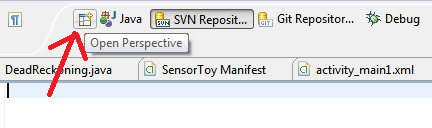
\includegraphics[height=10em]{new-perspective.png}
\end{center}
\caption{\label{fig:new-perspective}All of your active perspectives.}
\end{figure}

\begin{enumerate}
\item Click on the \textbf{Open Perspective} button at the top of your Eclipse window. (See Figure~\ref{fig:new-perspective}.)
\item Select \textbf{Other...} from the dropdown.
\item Select \textbf{SVN Repository Exploring} from the dialogue.
\item Switch to the new perspective tab that you just created.
\item Find the view labelled \textbf{SVN Repositories}. Right-click there and select \textbf{New \textgreater~Repository Location...}
\item Enter the URL:

\qquad \url{https://ecesvn.uwaterloo.ca/courses/ece155/w15} 
\item A dialog will pop up asking for your username and password. Use your Quest login. You should also check the \textbf{Save Password} box, otherwise Subclipse will ask you for your password whenever you navigate to a different folder. A word of warning if you do this: \textcolor{Red}{\textbf{On some systems, the password is stored as plain text. Don't use this option on shared computers!}}

On Linux-based systems, passwords are stored in \url{~/.subversion/auth/svn.simple}. On Windows, they are stored in \path{c:\Documents and Settings\your_username\Application Data\subversion\auth\svn.simple}.

\item You will be able to check your code into the folder groups/group-SSS-NN where SSS is your lab section number and NN is your group number. We will only mark your submission after you have committed your code to that folder.
\end{enumerate}

\paragraph{Getting files from the repository} In this course, we will provide you with sample code for some labs. You can find this good stuff in the repository's {\tt materials/} folder. You can view files in the repository by double-clicking them as normal. You can also download a local copy by right-clicking on a folder and selecting \textbf{Checkout...}. In the dialog, you can just click finish, and it will create a new project in your workspace that will contain all the files in the folder you checked out.

In the future, when you want to update your code to match the repository, you can do this by right-clicking on the top-level folder in your project and selecting \textbf{Team \textgreater~Update to HEAD}.

\paragraph{Adding your project to the repository} Once you have created a project, and you want to add it to the repository, follow these steps:

\begin{enumerate}
\item Right-click on the project and select \textbf{Team \textgreater~Share Project...}.
\item From the Repository Type dialog, select \textbf{SVN} click \textbf{Next}.
\item Make sure the repository you just added is selected and click \textbf{Next}.
\item Select \textbf{Use specified folder name}	and enter ``groups/group-SSS-NN/lab0-SSS-NN''. Then click \textbf{Finish}. 
\item This will add all of the files in your project to the current change-list and ask you to open the synchronization perspective.
\item You can say \textbf{No} on the synchronization perspective because we don't need it now.
\item At this point, your don't need to do anything more. Just right-click on the top-level folder in your project and select \textbf{Team \textgreater~Commit}.
\item In the future, when you make changes to your code, you can commit it to the server by right-clicking on the top-level folder and in the Java perspective selecting \textbf{Team \textgreater~Commit}.
\item Remember: if you add a new file, you will need to explicitly put it under version control by right clicking it and selecting \textbf{Team \textgreater~Add to Version Control}.
\end{enumerate}

\paragraph{Conflicts} While you are working on your code with your partner, sometimes you will modify the same file. Most of the time, Subversion is smart enough to detect that two changes are not on the same lines and will automatically merge these changes for you. However, sometimes you and your partner will edit the same lines. In this case, you have a conflict. When that happens, Subversion will not let you commit your changes. Here is how you fix it:

\begin{figure}[htbp]
\begin{center}
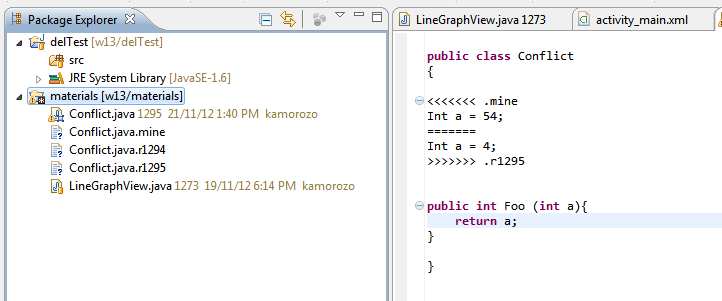
\includegraphics[width=\textwidth]{conflict.png}
\end{center}
\caption{\label{fig:conflict}Conflict Resolution.}
\end{figure}

\begin{enumerate}
\item You need to get the changes that are causing the conflict. You do this by right-clicking on the project and selecting \textbf{Team \textgreater~Update to HEAD}.
\item You will see a little square icon beside any files that have conflicts. Look at Conflict.java in figure \ref{fig:conflict}.
\item If you open the file, you will see the conflicting changes side by side in the code.
\item You should choose which version of each change to keep, and edit each conflicting file accordingly.
\item Once you are done, for each file with a conflict, you will need to right-click on it and select \textbf{Team \textgreater~Mark Resolved}.
\item This will bring up a dialog that will let you choose if you want to keep one of the existing versions of the file or your manual resolutions.
\item Once you have resolved all the conflicts, try to commit again.
\end{enumerate}

\section{Done?}
If you've finished early, it may be a good idea to go on to Lab 1. Being ahead of the game early in the term can really pay off later when things get busier!

%% \newpage
%% \section {Device Vendor IDs}

%% \begin{tabular}{l|l}
%% Company&USB Vendor ID\\
%% \hline
%% Acer &0502 \\
%% ASUS &0b05\\
%% Dell &413c\\
%% Foxconn &0489\\
%% Fujitsu &04c5\\
%% Fujitsu Toshiba &04c5\\
%% Garmin-Asus &091e\\
%% Google &18d1\\
%% Hisense &109b\\
%% HTC &0bb4\\
%% Huawei &12d1\\
%% K-Touch &24e3\\
%% KT Tech &2116\\
%% Kyocera &0482\\
%% Lenovo &17ef\\
%% LG &1004\\
%% Motorola &22b8\\
%% NEC &0409\\
%% Nook &2080\\
%% Nvidia &0955\\
%% OTGV &2257\\
%% Pantech &10a9\\
%% Pegatron &1d4d\\
%% Philips &0471\\
%% PMC-Sierra &04da\\
%% Qualcomm &05c6\\
%% SK Telesys &1f53\\
%% Samsung &04e8\\
%% Sharp &04dd\\
%% Sony &054c\\
%% Sony Ericsson &0fce\\
%% Teleepoch &2340\\
%% Toshiba &0930\\
%% ZTE &19d2\\
%% \end{tabular}

\end{document}






